\documentclass[12pt, a4paper]{article}

\usepackage{graphicx}
\usepackage{xcolor}
\usepackage{float}
\usepackage{svg}
\usepackage[colorlinks=true, linkcolor=black, urlcolor=blue, citecolor=green]{hyperref}
\usepackage{enumitem}
\usepackage[italian]{babel}
\usepackage{lastpage}  % Pacchetto per ottenere il numero totale delle pagine
\usepackage{fancyhdr}  % Pacchetto per personalizzare l'intestazione e il piè di pagina
\usepackage[margin=1in]{geometry}
\usepackage{array}
\newcolumntype{C}[1]{>{\centering\arraybackslash}p{#1}}
\newcolumntype{L}[1]{>{\raggedright\arraybackslash}p{#1}}
\graphicspath{ {images/} {../shared/images/} }
\definecolor{unipd}{HTML}{B5121B}

\addto\captionsitalian{\renewcommand{\contentsname}{Indice}}


\pagestyle{fancy}% Imposta lo stile di pagina su "fancy"
\fancyhf{}% Cancella intestazioni e piè di pagina
\fancyfoot[C]{\thepage{} di \pageref{LastPage}} % Imposta il piè di pagina centrale come "numero pagina di totale pagine"
\renewcommand{\headrulewidth}{0pt} % Imposta la larghezza della linea di intestazione a 0 punti

% COMANDI PER CONTATORI
\newcounter{uccounter}
\newcommand{\uc}[2]{%
  \refstepcounter{uccounter}%
  \addcontentsline{toc}{subsubsection}{UC\arabic{uccounter}\ - #1}%
  \subsubsection*{\label{#2}\textbf{UC\arabic{uccounter}\ - #1}}%
}

\newcounter{subuccounter}[uccounter]
\newcommand{\subuc}[2]{%
  \refstepcounter{subuccounter}%
  \addcontentsline{toc}{subsubsection}{UC\arabic{uccounter}.\arabic{subuccounter}\ - #1}%
  \subsubsection*{\label{#2}\textbf{UC\arabic{uccounter}.\arabic{subuccounter}\ - #1}}%
}

\newcounter{subsubuccounter}[subuccounter]
\newcommand{\subsubuc}[2]{%
  \refstepcounter{subsubuccounter}%
  \addcontentsline{toc}{subsubsection}{UC\arabic{uccounter}.\arabic{subuccounter}.\arabic{subsubuccounter}\ - #1}%
  \subsubsection*{\label{#2}\textbf{UC\arabic{uccounter}.\arabic{subuccounter}.\arabic{subsubuccounter}\ - #1}}%
}

\newcounter{subsubsubuccounter}[subsubuccounter]
\newcommand{\subsubsubuc}[2]{%
  \refstepcounter{subsubsubuccounter}%
  \addcontentsline{toc}{subsubsection}{UC\arabic{uccounter}.\arabic{subuccounter}.\arabic{subsubuccounter}.\arabic{subsubsubuccounter}\ - #1}%
  \subsubsection*{\label{#2}\textbf{UC\arabic{uccounter}.\arabic{subuccounter}.\arabic{subsubuccounter}.\arabic{subsubsubuccounter}\ - #1}}%
}

% \newcommand{\data}{GG mese AAAA}
\newcommand{\titolo}{Analisi dei Requisiti}
% \newcommand{\responsabile}{Responsabile}
\newcommand{\verificatore}{
    & Davide Martinelli \\
    & Nome2 Cognome2 \\
    & Nome3 Cognome3 \\
}
\newcommand{\redattore}{
    & Nome1 Cognome1 \\
    & Nome2 Cognome2 \\
    & Nome3 Cognome3 \\
}
% \newcommand{\uso}{Interno/Esterno}
\newcommand{\destinatari }{
    & Tullio Vardanega \\
    & Riccardo Cardin \\
    & Vimar S.p.A. \\
    & Gruppo PEBKAC
}
\newcommand{\abstractcontent}{abstract ...}

\begin{document}

\begin{minipage}[]{0.3\textwidth}
\includesvg[width=\linewidth]{pebkac.svg} 
\end{minipage}
\hspace{0.1\textwidth}
\begin{minipage}[]{0.6\textwidth}
  {\Large \textbf{PEBKAC}} \\
  Email: \href{mailto:pebkacswe@gmail.com}{pebkacswe@gmail.com} \\
  Gruppo: 11
\end{minipage}

\bigskip

\begin{minipage}[]{0.3\textwidth}
\includesvg[width=\linewidth]{logo_unipd.svg} 
\end{minipage}
\hspace{0.1\textwidth}
\begin{minipage}[]{0.6\textwidth}
  \textcolor{unipd}{
    \textbf{Università degli Studi di Padova} \\
    Corso di Laurea: Informatica \\
    Corso: Ingegneria del Software \\
    Anno Accademico: 2024/2025
  }
\end{minipage}


\bigskip
\bigskip
\bigskip
\begin{center}
  \Huge\textbf{Verbale Interno}

  \Large\textbf{\data}
\end{center}

\bigskip


\begin{center}
\textbf{Informazioni sul documento}: \\
\vspace{0.5cm}

\begin{tabular}{r|l}
    \textbf{Responsabile} & Tommaso Zocche \\ 
    \textbf{Verificatore} & Alessandro Benin \\ 
    \textbf{Redattore} & Tommaso Zocche \\ 
    \textbf{Uso} & Interno \\ 
    \textbf{Destinatari} & Tullio Vardanega \\ & Riccardo Cardin \\ 
\end{tabular}

\vfill

\textbf{Abstract}: \\
\vspace{0.5cm}
L'obiettivo dell'incontro è stato definire l'ordine di preferenza dei capitolati a seguito degli incontri avuti con le aziende interessate e iniziare a redigere il prospetto orario del gruppo.
\end{center}


\bigskip
\newpage

\section*{Registro delle modifiche}
\begin{table}[H]
    \begin{tabular}{|c|c|c|c|p{5cm}|}
        \hline
         \textbf{Versione} &  \textbf{Data} &  \textbf{Autore} &  \textbf{Ruolo} & \textbf{Descrizione} \\
          \hline
          &  &  & Responsabile & Approvazione e rilascio\\
          \hline
          0.1.0 & 17/11/2024 & Alessandro Benin & Verificatore  & Verificato \\
          \hline
          0.0.1 & 13/11/2024 & Derek Gusatto & Amministratore  & Stesura iniziale \\
          \hline
    \end{tabular}
\end{table}
\newpage
\tableofcontents
\newpage
%LISTA FIGURE
\listoffigures 
\newpage
%LISTA TABELLE
\listoftables
\newpage
\section{Introduzione}
Questo documento mira a garantire chiarezza e uniformità nella terminologia utilizzata all'interno della documentazione del progetto, riducendo al minimo le ambiguità o potenziali incomprensioni. A tal fine, include un glossario che fornisce definizioni precise per i termini specifici del dominio d'uso.
Per facilitare la consultazione, i termini sono organizzati in ordine alfabetico, consentendo una navigazione semplice e immediata. Inoltre, in tutti gli altri documenti del progetto, i termini presenti nel Glossario saranno identificati da un simbolo di riferimento, rappresentato da una ``G" in pedice.
\newpage
\section{Descrizione del Prodotto}
\subsection{Obiettivo fissato}
L’obiettivo del progetto é quello di fornire al Proponente un’app in grado di fornire supporto in tempo reale agli installatori di dispositivi offerti dall’azienda allo scopo di agevolare e velocizzare la raccolta di informazioni richieste. Per rendere efficiente e veloce la raccolta di informazioni, l’azienda sceglie di basare la ricerca principalmente sull’interrogazione di LLM. La soluzione potrà essere realizzata tramite un sistema di chat dove l’utente, tramite linguaggio naturale, fa delle richieste ed ottiene delle risposte da un’intelligenza artificiale.

\subsection{Funzioni del prodotto}
Il software deve essere in grado di recuperare informazioni dal sito web di Vimar e indicizzarle in un database vettoriale\textsubscript{G} dal quale un LLM possa ricavare le informazioni per rispondere alle domande poste dagli installatori.
Secondariamente il software deve permettere la gestione di queste chat.

\subsection{Tecnologie  e analisi della struttura di progetto} 
\subsubsection{Vincoli tecnologici}
I vincoli tecnologici sono i seguenti:
\begin{itemize}
    \item L’infrastruttura Cloud deve usare Docker con docker-compose al fine di far valere il
    principio di infrastructure as code.
    \item Il repository di lavoro deve essere versionato tramite Git e deve essere pubblicamente
    accessibile e per i sorgenti la licenza dovrà essere open
    source
    \item La parte di intelligenza artificiale dovrà fare uso dell’approccio RAG e usare un modello LLM
\end{itemize}
Inoltre vengono suggerite le seguenti tecnologie da utilizzare:
\begin{itemize}
    \item A livello di applicativo web responsive, si consigliano framework come Flask (Python), Angular
    (TypeScript) o VueJS per lo sviluppo front-end.
    \item Per lo sviluppo (es. API, business-logic) è fortemente consigliato l’utilizzo di Python come
    linguaggio di programmazione, vista la semplicità di utilizzo e di apprendimento.
    \item Per il componente di estrazione e reperimento delle informazioni dal sito web, si consigliano
    librerie di Web Scraping e OCR, come ad esempio Scrapy e OCRmyPDF.
    \item A livello di database, si consiglia l’utilizzo di database relazionali come PostgreSQL per
    immagazzinare i dati, unito all’uso dell’estensione pgvector per realizzare indici vettoriali (cfr.
    embeddings \#1, embeddings \#2) da sfruttare col componente di interrogazione. In alternativa si
    possono utilizzare database NoSQL come TimescaleDB o InfluxDB.
    \item Per il componente di interrogazione si consiglia di lavorare con modelli open source di LLM come
    ad esempio Llama 3.1, Mistral, Bert o Phi. Il sito di HuggingFace riporta anche una lista di LLM
    (sotto al tab Retrieval) che usino il RAG.
    \item In ottica di soluzione a container con sviluppo su AWS, si consiglia di utilizzare il servizio AWS
    LightSail (ref. guida a LightSail Containers) oppure AWS EC2 (Elastic Compute Cloud).
    \item Nell’ambito del software development lifecycle, si raccomanda l’utilizzo di una CI (es. GitHub
    Runners) per automatizzare l’esecuzione di test e l’analisi statica del codice.
    \item Nell’ambito dello sviluppo software, si consiglia l’utilizzo di GitHub Copilot (vedi GitHub Student
    Pack) o Amazon Q (versione gratuita).
\end{itemize}

\subsection{Caratteristiche utente}
Gli utenti principali di questo prodotto software sono gli installatori, professionisti che si occupano della progettazione, messa in funzione e manutenzione di un impianto elettrico e domotico, che andranno a interrogare il chatbot per reperire informazioni testuali e grafiche sui prodotti Vimar presenti all'interno del sito ufficiale. 
\newpage
\section{Casi d'uso}
\subsection{Scopo}
In questa sezione si vuole elencare e descrivere tutti i casi d'uso individuati dall'analisi del \textit{capitolato}\textsubscript{G} e dalle interazioni con il Proponente. Inoltre si vogliono individuare gli attori\textsubscript{G} e le funzionalità che questi possono svolgere. Ogni caso d'uso è identificato univocamente come descritto in Norme di Progetto V1.0.0,  §3.2.2 Analisi dei Requisiti.

\subsection{Attori}
Gli attori presi in considerazione nel prodotto che realizzeremo includono:
\begin{itemize}
    \item \textbf{Installatore}: Un utente non autenticato che consulta il \textit{sistema}\textsubscript{G} per ottenere informazioni tecniche e configurare i dispositivi.; 
    \item \textbf{\textit{Amministratore}\textsubscript{G}}: Un utente autenticato che accede alla \textit{dashboard}\textsubscript{G} protetta per monitorare l’uso del \textit{sistema}\textsubscript{G}, visualizzare statistiche e gestire il \textit{feedback}\textsubscript{G} degli installatori.
\end{itemize}
\begin{figure}[H]
\centering

\includegraphics[height=5cm]{contents/casi_duso/png/attori.png}
\caption{Attori}
% \label{fig:UC1a}
\end{figure}

\subsection{Elenco dei casi d'uso}

\uc{Creazione \textit{conversazione libera}\textsubscript{G}}{conv_libera}
\begin{itemize}
    \item \textbf{Attori coinvolti}: Installatore;
    \item \textbf{Descrizione}: L’installatore desidera interrogare il \textit{sistema}\textsubscript{G}, quindi crea una nuova \textit{conversazione libera}\textsubscript{G} per richiedere le informazioni a lui necessarie tramite domande poste in linguaggio naturale;
    \item \textbf{Precondizioni}: L’installatore ha accesso all’\textit{interfaccia web}\textsubscript{G} del \textit{sistema}\textsubscript{G};
    \item \textbf{Postcondizioni}: Il \textit{sistema}\textsubscript{G} crea una nuova \textit{conversazione libera}\textsubscript{G} a cui puó accedere l’installatore, dove potrà porre liberamente domande in linguaggio naturale al \textit{sistema}\textsubscript{G};
    \item \textbf{Scenario principale}:
    \begin{enumerate}
    \item L’installatore accede all’\textit{interfaccia web}\textsubscript{G} di Vimar GENIALE;
    \item Richiede la creazione di una nuova conversazione in modalità libera;
    \item Il \textit{sistema}\textsubscript{G} esegue la creazione della nuova conversazione nella modalità desiderata dall’utente;
    \item  L’installatore accede alla nuova conversazione.
    \end{enumerate}
    \item \textbf{Estensioni}: UC2 - Raggiungimento limite di conversazioni;
\end{itemize}
\begin{figure}[H]
\centering
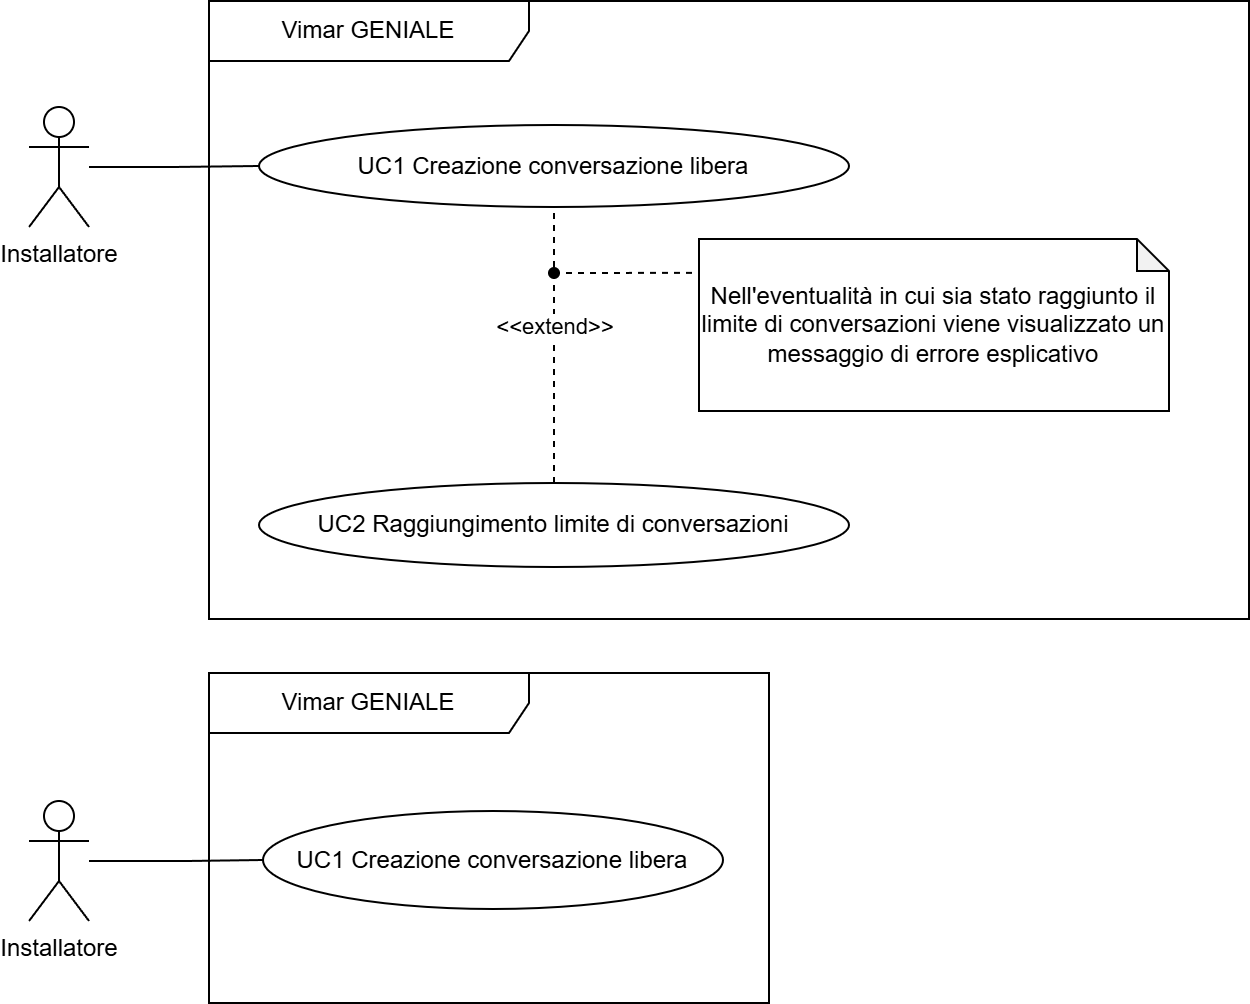
\includegraphics[width=0.8\textwidth]{contents/casi_duso/png/UC1.png}
\caption{UC1, UC2 - Creazione \textit{conversazione libera}\textsubscript{G}}
% \label{fig:UC1a}
\end{figure}

\uc{Raggiungimento limite di conversazioni}{limite_conv}
\begin{itemize}
    \item \textbf{Attori coinvolti}: Installatore;
    \item \textbf{Descrizione}: L’installatore desidera interrogare il \textit{sistema}\textsubscript{G}, ma quando prova a creare una nuova conversazione per richiedere le informazioni a lui necessarie, supera il limite massimo di conversazioni supportate;
    \item \textbf{Precondizioni}: 
        \begin{itemize}
            \item L’installatore ha accesso all’\textit{interfaccia web}\textsubscript{G} del \textit{sistema}\textsubscript{G};
            \item Il numero di conversazioni memorizzate nel \textit{sistema}\textsubscript{G} supera il limite massimo supportato;
        \end{itemize}
    \item \textbf{Postcondizioni}:  Il \textit{sistema}\textsubscript{G} restituisce una risposta che indica il motivo per cui si è verificato l’errore;
    \item \textbf{Scenario principale}:
    \begin{enumerate}
    \item L’installatore accede all’\textit{interfaccia web}\textsubscript{G} di Vimar GENIALE;
    \item Richiede la creazione di una nuova conversazione, nonostante siano già esistenti un numero di conversazioni che raggiunge il limite;
    \item Il \textit{sistema}\textsubscript{G} elabora la richiesta e fornisce una risposta che spiega la causa dell'errore riscontrato;
    \item L’installatore visualizza le informazioni sull’errore che si è verificato.
    \end{enumerate}
\end{itemize}



\uc{Salvataggio conversazione}{salvataggio_conv}
\begin{itemize}
    \item \textbf{Attori coinvolti}: Installatore;
    \item \textbf{Descrizione}: L’installatore, prima di chiudere l’applicativo, desidera salvare le conversazioni memorizzate attualmente all’interno del \textit{sistema}\textsubscript{G}, per poterle utilizzare nuovamente dal punto in cui ha concluso in precedenza alla prossima apertura dell’applicativo;
    \item \textbf{Precondizioni}: 
        \begin{itemize}
            \item L’installatore ha accesso all’\textit{interfaccia web}\textsubscript{G} del \textit{sistema}\textsubscript{G};
            \item Sono presenti nel \textit{sistema}\textsubscript{G} un numero consentito di conversazioni;
        \end{itemize}
    \item \textbf{Postcondizioni}: Il \textit{sistema}\textsubscript{G} salva le conversazioni memorizzate attualmente all’interno del \textit{sistema}\textsubscript{G};
    \item \textbf{Scenario principale}:
    \begin{enumerate}
    \item L’installatore accede all’\textit{interfaccia web}\textsubscript{G} di Vimar GENIALE;
    \item Richiede il salvataggio delle conversazioni esistenti al momento, prima di effettuare la chiusura dell’applicativo;
    \item Il \textit{sistema}\textsubscript{G} effettua il salvataggio e fornisce una risposta che conferma il completamento dell’operazione;
    \item L’installatore visualizza il messaggio di conferma dell’avvenuto salvataggio.
    \end{enumerate}
    \item \textbf{Estensioni}: UC4 - Salvataggio conversazione vuota
\end{itemize}
\begin{figure}[H]
\centering
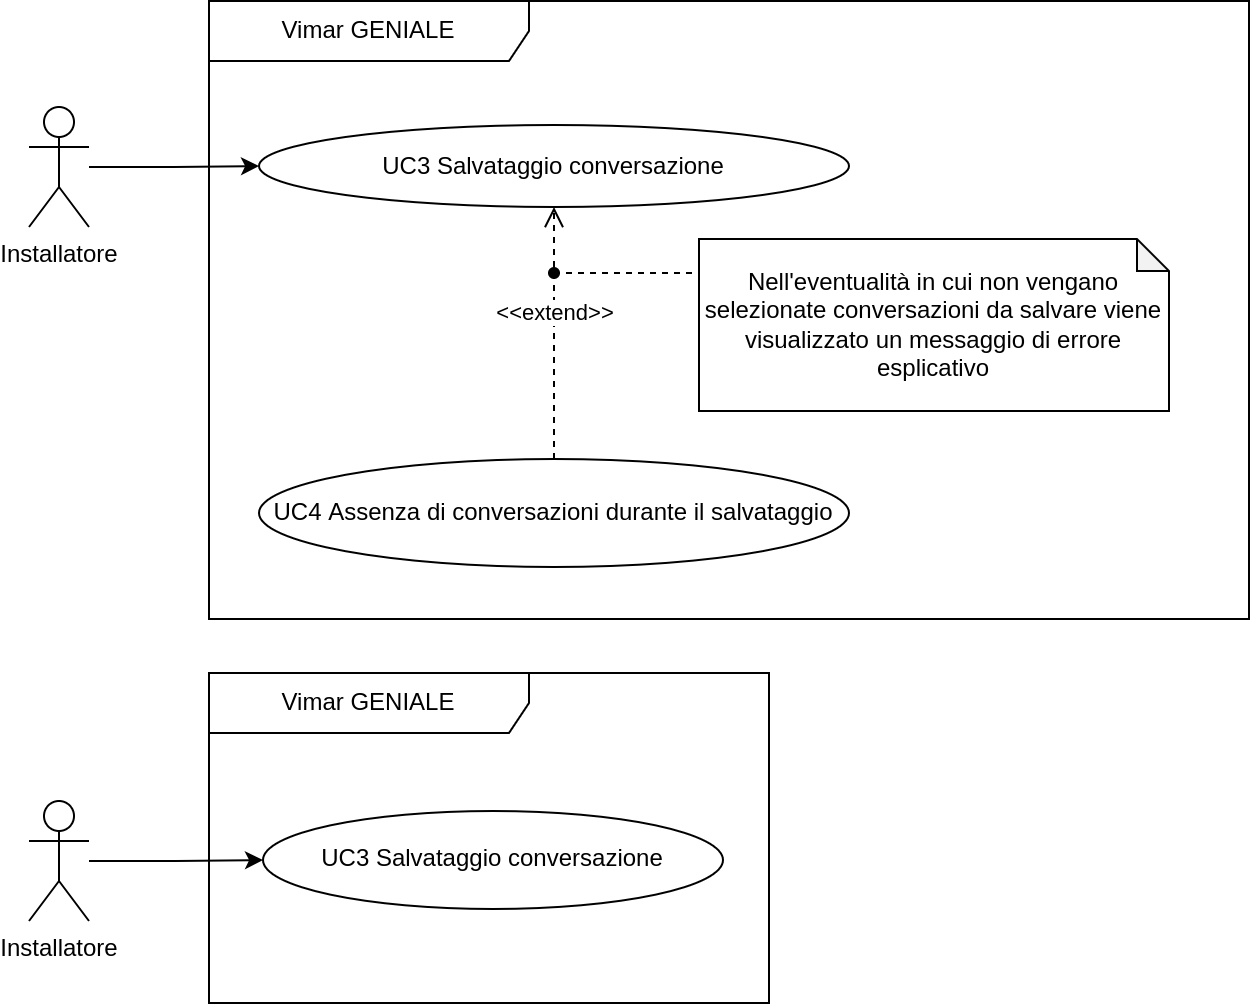
\includegraphics[width=0.8\textwidth]{contents/casi_duso/png/UC3.png}
\caption{UC3, UC4 - Salvataggio conversazione}
% \label{fig:UC1a}
\end{figure}

\uc{Salvataggio conversazione vuota}{assenza_conv}
\begin{itemize}
    \item \textbf{Attori coinvolti}: Installatore;
    \item \textbf{Descrizione}: L’installatore tenta di salvare una o più conversazioni vuote;
    \item \textbf{Precondizioni}: 
        \begin{itemize}
            \item L’installatore ha accesso all’\textit{interfaccia web}\textsubscript{G} del \textit{sistema}\textsubscript{G};
            \item L'installatore crea una nuova \textit{conversazione libera}\textsubscript{G} e poi non fa nessuna domanda.
        \end{itemize}
    \item \textbf{Postcondizioni}: Il \textit{sistema}\textsubscript{G} restituisce una risposta che indica il motivo per cui si è verificato l’errore;
    \item \textbf{Scenario principale}:
    \begin{enumerate}
    \item L’installatore accede all’\textit{interfaccia web}\textsubscript{G} di Vimar GENIALE;
    \item L'installatore crea una nuova conversazione, ma non pone nessuna domanda.
    \item Richiede il salvataggio di una o più conversazioni;
    \item Il \textit{sistema}\textsubscript{G} elabora la richiesta e fornisce una risposta che spiega la causa dell'errore riscontrato;
    \item L’installatore visualizza le informazioni sull’errore che si è verificato.
    \end{enumerate}
\end{itemize}



\uc{Cancellazione conversazione}{cancellazione_conv}
\begin{itemize}
    \item \textbf{Attori coinvolti}: Installatore;
    \item \textbf{Descrizione}: L’installatore desidera eliminare una conversazione esistente, in quanto non è ritenuta più necessaria al suo scopo;
    \item \textbf{Precondizioni}: 
        \begin{itemize}
            \item L’installatore ha accesso all’\textit{interfaccia web}\textsubscript{G} del \textit{sistema}\textsubscript{G};
            \item L’installatore ha accesso ad una conversazione memorizzata nel \textit{sistema}\textsubscript{G};
        \end{itemize}
    \item \textbf{Postcondizioni}: Il \textit{sistema}\textsubscript{G} elimina la conversazione non ritenuta più necessaria dall’installatore.
    \item \textbf{Scenario principale}:
    \begin{enumerate}
    \item L’installatore accede all’\textit{interfaccia web}\textsubscript{G} di Vimar GENIALE;
    \item Richiede l’eliminazione di una conversazione, in quanto ha raggiunto il suo scopo e non è più utile;
    \item Il \textit{sistema}\textsubscript{G} effettua l’eliminazione e fornisce una risposta che conferma il completamento dell’operazione;
    \item L’installatore visualizza il messaggio di conferma dell’avvenuta cancellazione.
    \end{enumerate}
\end{itemize}
\begin{figure}[H]
\centering
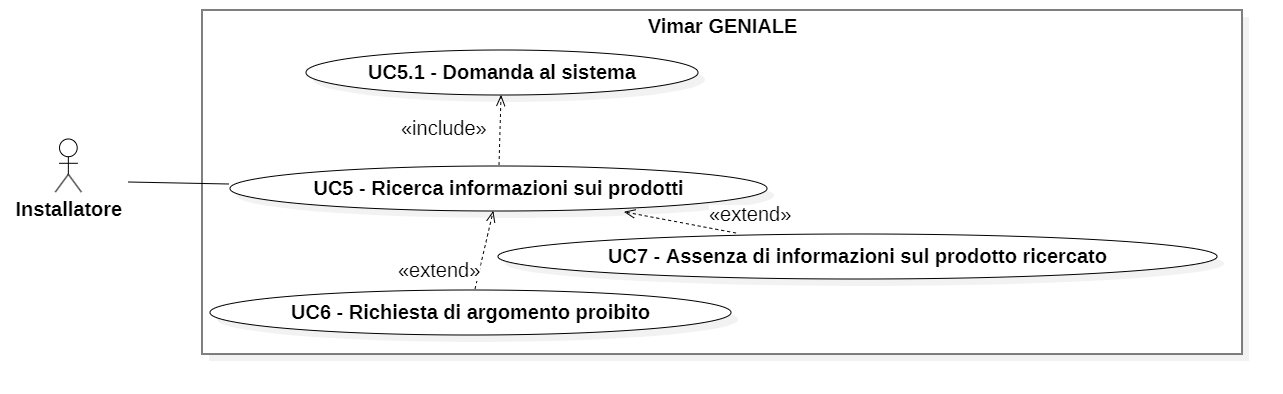
\includegraphics[width=0.8\textwidth]{contents/casi_duso/png/UC5.png}
\caption{UC5 - Cancellazione conversazione}
% \label{fig:UC1a}
\end{figure}


\uc{Ricerca informazioni sui prodotti con \textit{conversazione libera}\textsubscript{G}}{ricerca_info_prodotti}
\begin{itemize}
    \item \textbf{Attori coinvolti}: Installatore;
    \item \textbf{Descrizione}: L’installatore interroga il \textit{sistema}\textsubscript{G} per ottenere informazioni dettagliate su un prodotto specifico, come schemi elettrici, dati tecnici e manuali;
    \item \textbf{Precondizioni}: 
        \begin{itemize}
            \item L’installatore ha accesso all’\textit{interfaccia web}\textsubscript{G} del \textit{sistema}\textsubscript{G};
            \item L’installatore ha accesso ad una conversazione memorizzabile nel \textit{sistema}\textsubscript{G};
            \item Il prodotto richiesto è registrato nel \textit{sistema}\textsubscript{G} e le informazioni sono correttamente indicizzate.
        \end{itemize}
    \item \textbf{Postcondizioni}: Il \textit{sistema}\textsubscript{G} restituisce le informazioni richieste, incluse le descrizioni del prodotto, schemi elettrici e manuali di configurazione;
    \item \textbf{Scenario principale}:
    \begin{enumerate}
    \item L’installatore accede all’\textit{interfaccia web}\textsubscript{G} di Vimar GENIALE;
    \item Inserisce una domanda o una parola chiave relativa ad un prodotto specifico;
    \item Il \textit{sistema}\textsubscript{G} esegue la ricerca nel \textit{database}\textsubscript{G} le informazioni necessarie a fornire sufficiente contesto al \textit{LLM}\textsubscript{G}.
    \end{enumerate}
    \item \textbf{Inclusioni}: UC18 - Digitare la domanda.
    \item \textbf{Estensioni}: 
    \begin{itemize}
        \item UC8 - Assenza di informazioni sul prodotto ricercato;
        \item UC15 - Richiesta di argomento proibito
    \end{itemize}

\end{itemize}
\begin{figure}[H]
\centering
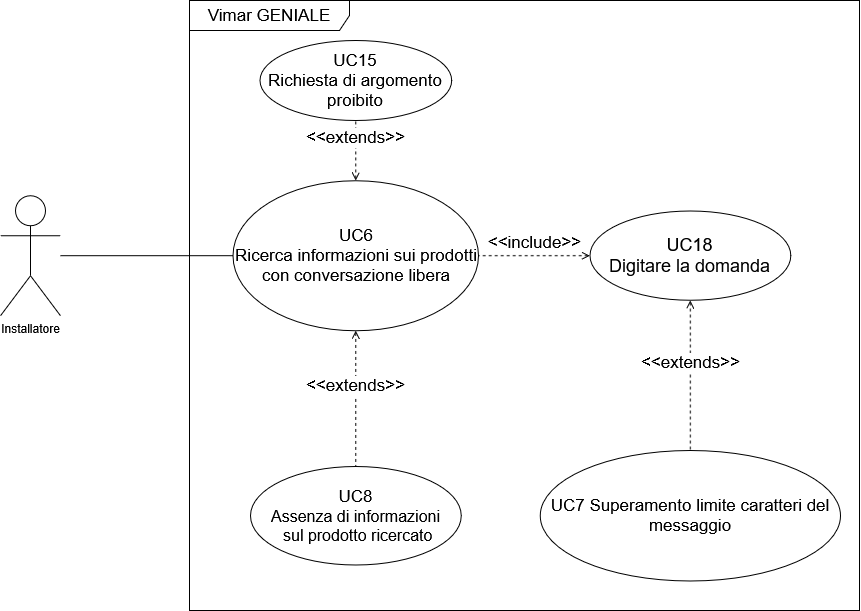
\includegraphics[width=0.8\textwidth]{contents/casi_duso/png/UC6.png}
\caption{UC6, UC7, UC8, UC15, UC16, UC18 - Ricerca informazioni sui prodotti con \textit{conversazione libera}\textsubscript{G}}
\end{figure}


\uc{Superamento limite caratteri del messaggio}{superamento_limite_caratteri}
\begin{itemize}
    \item \textbf{Attori coinvolti}: Installatore;
    \item \textbf{Descrizione}: L’installatore, quando interroga il \textit{sistema}\textsubscript{G} per ottenere informazioni, supera il limite di caratteri che possono essere utilizzati per effettuare la richiesta;
    \item \textbf{Precondizioni}: 
        \begin{itemize}
            \item L’installatore ha accesso all’\textit{interfaccia web}\textsubscript{G} del \textit{sistema}\textsubscript{G};
            \item L’installatore ha accesso ad una conversazione memorizzabile nel \textit{sistema}\textsubscript{G};
            \item La domanda posta supera il limite massimo di caratteri consentiti.
        \end{itemize}
    \item \textbf{Postcondizioni}: Il \textit{sistema}\textsubscript{G} restituisce una risposta che indica il motivo per cui si è verificato l’errore;
    \item \textbf{Scenario principale}:
    \begin{enumerate}
    \item L’installatore accede all’\textit{interfaccia web}\textsubscript{G} di Vimar GENIALE;
    \item Inserisce una domanda o una parola chiave relativa ad un prodotto specifico, superando il limite massimo consentito di caratteri;
    \item Il \textit{sistema}\textsubscript{G} elabora la richiesta e fornisce una risposta che spiega la causa dell'errore riscontrato;
    \item L’installatore visualizza le informazioni sull’errore che si è verificato.
    \end{enumerate}
\end{itemize}


\uc{Assenza di informazioni sul prodotto ricercato}{assenza_info_prodotto}
\begin{itemize}
    \item \textbf{Attori coinvolti}: Installatore;
    \item \textbf{Descrizione}: L’installatore interroga il \textit{sistema}\textsubscript{G} per ottenere informazioni dettagliate su un prodotto specifico, ma il \textit{sistema}\textsubscript{G} non è in grado di trovare nessuna informazione relativa ad esso;
    \item \textbf{Precondizioni}: 
        \begin{itemize}
            \item L’installatore ha accesso all’\textit{interfaccia web}\textsubscript{G} del \textit{sistema}\textsubscript{G};
            \item L’installatore ha accesso ad una conversazione memorizzabile nel \textit{sistema}\textsubscript{G};
            \item L’installatore pone una domanda al \textit{sistema}\textsubscript{G};
            \item Il \textit{sistema}\textsubscript{G} non è in possesso di alcuna informazione relativa al prodotto ricercato.
        \end{itemize}
    \item \textbf{Postcondizioni}: Il \textit{sistema}\textsubscript{G} restituisce una risposta che indica il motivo per cui si è verificato l’errore;
    \item \textbf{Scenario principale}:
    \begin{enumerate}
    \item L’installatore accede all’\textit{interfaccia web}\textsubscript{G} di Vimar GENIALE;
    \item Inserisce una domanda o una parola chiave relativa ad un prodotto specifico;
    \item Il \textit{sistema}\textsubscript{G} elabora la richiesta e fornisce una risposta che spiega la causa dell'errore riscontrato;
    \item L’installatore visualizza le informazioni sull’errore che si è verificato.
    \end{enumerate}
\end{itemize}


\uc{Visualizzazione storico dei messaggi}{visualizzazione_storico_messaggi}
\begin{itemize}
    \item \textbf{Attori coinvolti}: Installatore;
    \item \textbf{Descrizione}: L’installatore, avendo la necessità di riesaminare le risposte ricevute alle domande poste in precedenza, richiede al \textit{sistema}\textsubscript{G} di mostrare uno storico dei messaggi della conversazione attuale;
    \item \textbf{Precondizioni}: 
        \begin{itemize}
            \item L’installatore ha accesso all’\textit{interfaccia web}\textsubscript{G} del \textit{sistema}\textsubscript{G};
            \item L’installatore ha accesso ad una conversazione memorizzabile nel \textit{sistema}\textsubscript{G};
            \item La conversazione attuale contiene dei messaggi che sono stati scambiati in precedenza.
        \end{itemize}
    \item \textbf{Postcondizioni}: Il \textit{sistema}\textsubscript{G} ritorna lo storico dei messaggi della conversazione attuale.
    \item \textbf{Scenario principale}:
    \begin{enumerate}
    \item L’installatore accede all’\textit{interfaccia web}\textsubscript{G} di Vimar GENIALE;
    \item Accede ad una conversazione presente nel \textit{sistema}\textsubscript{G} e richiede di visualizzarne uno storico dei messaggi;
    \item Il \textit{sistema}\textsubscript{G} elabora la richiesta e fornisce lo storico dei messaggi della conversazione attuale;
    \item L’installatore visualizza i messaggi scambiati in precedenza nella conversazione corrente.
    \end{enumerate}
    \item \textbf{Estensioni}: UC10 - Mancanza messaggi pregressi nella conversazione
\end{itemize}
\begin{figure}[H]
\centering
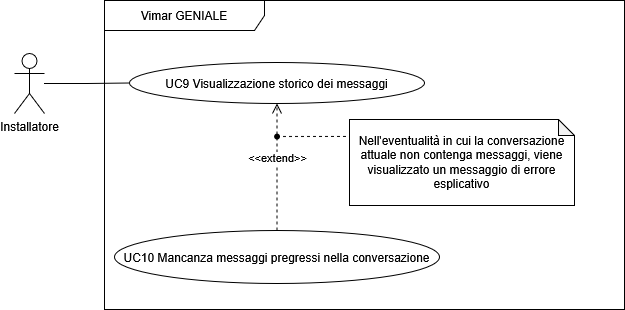
\includegraphics[width=0.8\textwidth]{contents/casi_duso/png/UC9.png}
\caption{UC9, UC10 - Visualizzazione storico dei messaggi}
% \label{fig:UC1a}
\end{figure}

\uc{Mancanza messaggi pregressi nella conversazione}{mancanza_messaggi_pregressi}
\begin{itemize}
    \item \textbf{Attori coinvolti}: Installatore;
    \item \textbf{Descrizione}: L’installatore richiede di visualizzare lo storico dei messaggi di una conversazione, ma non ci sono messaggi pregressi nella conversazione attuale;
    \item \textbf{Precondizioni}: 
        \begin{itemize}
            \item L’installatore ha accesso all’\textit{interfaccia web}\textsubscript{G} del \textit{sistema}\textsubscript{G};
            \item L’installatore ha accesso ad una conversazione memorizzabile nel \textit{sistema}\textsubscript{G};
            \item La conversazione attuale non contiene messaggi scambiati in precedenza.
        \end{itemize}
    \item \textbf{Postcondizioni}: Il \textit{sistema}\textsubscript{G} restituisce una risposta che indica l’assenza di messaggi pregressi nella conversazione attuale;
    \item \textbf{Scenario principale}:
    \begin{enumerate}
    \item L’installatore accede all’\textit{interfaccia web}\textsubscript{G} di Vimar GENIALE;
    \item Accede ad una conversazione presente nel \textit{sistema}\textsubscript{G} e richiede di visualizzarne uno storico dei messaggi;
    \item Il \textit{sistema}\textsubscript{G} elabora la richiesta e fornisce una risposta che indica l’assenza di messaggi pregressi nella conversazione attuale;
    \item L’installatore visualizza il messaggio che indica l’assenza di messaggi pregressi.
    \end{enumerate}
\end{itemize}



\uc{Fornitura di \textit{feedback}\textsubscript{G} sulla risposta del \textit{sistema}\textsubscript{G} ad interrogazione}{fornitura_feedback}
\begin{itemize}
    \item \textbf{Attori coinvolti}: Installatore;
    \item \textbf{Descrizione}: L’installatore, a seguito dell’interrogazione del \textit{sistema}\textsubscript{G} per ottenere informazioni, desidera fornire un \textit{feedback}\textsubscript{G} che indichi se la risposta ricevuta sia corretta o meno;
    \item \textbf{Precondizioni}: 
        \begin{itemize}
            \item L’installatore ha accesso all’\textit{interfaccia web}\textsubscript{G} del \textit{sistema}\textsubscript{G};
            \item L’installatore ha accesso ad una conversazione memorizzabile nel \textit{sistema}\textsubscript{G};
            \item Il \textit{sistema}\textsubscript{G} fornisce una risposta ad un’interrogazione da parte dell’installatore.
        \end{itemize}
    \item \textbf{Postcondizioni}: L’installatore, dopo aver esaminato la risposta ricevuta, fornisce un riscontro sulla correttezza di quest’ultima che verrà registrato dal \textit{sistema}\textsubscript{G};
    \item \textbf{Scenario principale}:
    \begin{enumerate}
    \item L’installatore accede all’\textit{interfaccia web}\textsubscript{G} di Vimar GENIALE;
    \item Inserisce una domanda o una parola chiave relativa ad un prodotto specifico;
    \item Il \textit{sistema}\textsubscript{G} esegue la ricerca nel \textit{database}\textsubscript{G} dei prodotti e restituisce una risposta che include informazioni dettagliate come schemi, descrizioni e manuali;
    \item L’installatore visualizza le informazioni fornite e, dopo aver verificato la correttezza delle informazioni ricevute, fornisce un \textit{feedback}\textsubscript{G} sulla risposta al \textit{sistema}\textsubscript{G};
    \item Il \textit{sistema}\textsubscript{G} registra il \textit{feedback}\textsubscript{G} ricevuto dall’installatore.
    \end{enumerate}
\end{itemize}
\begin{figure}[H]
\centering
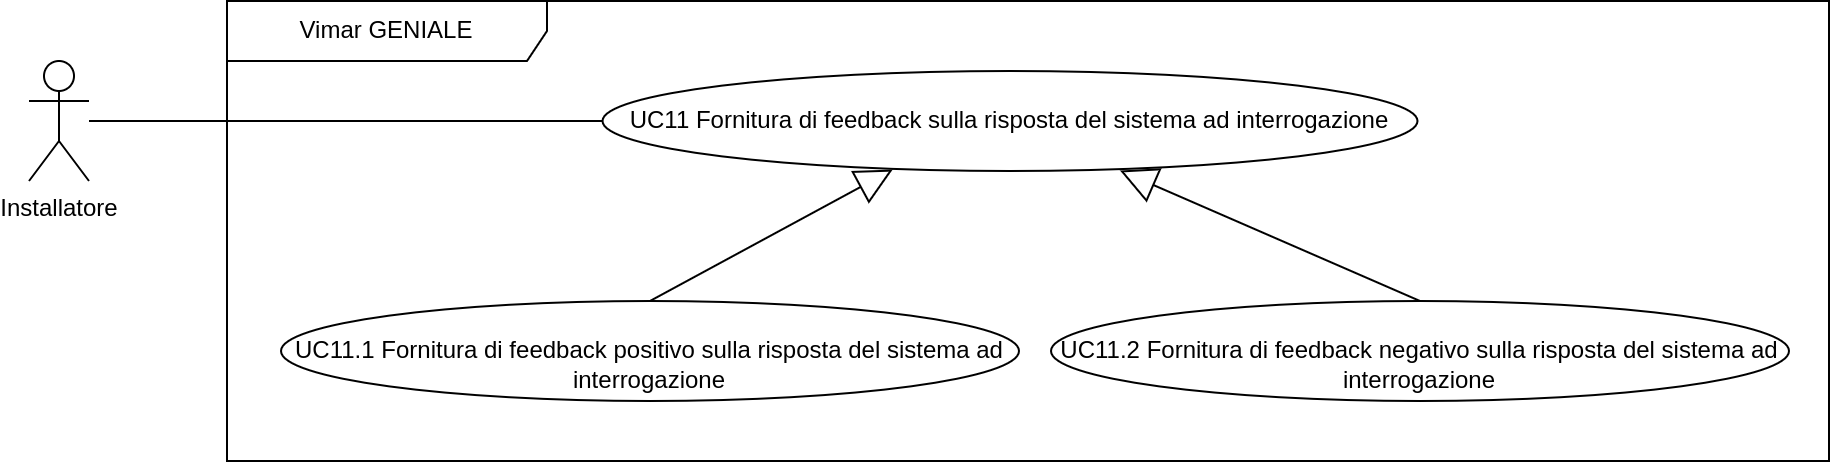
\includegraphics[width=0.8\textwidth]{contents/casi_duso/png/UC11.png}
\caption{UC11, UC11.1, UC11.2 - Fornitura di \textit{feedback}\textsubscript{G} sulla risposta del \textit{sistema}\textsubscript{G} ad interrogazione}
% \label{fig:UC1a}
\end{figure}

\subuc{Fornitura di \textit{feedback}\textsubscript{G} positivo sulla risposta del \textit{sistema}\textsubscript{G} ad interrogazione}{feedback_positivo}
\begin{itemize}
    \item \textbf{Attori coinvolti}: Installatore;
    \item \textbf{Descrizione}: L’installatore, a seguito dell’interrogazione del \textit{sistema}\textsubscript{G} per ottenere informazioni, desidera fornire un \textit{feedback}\textsubscript{G} che indichi che la risposta ricevuta è corretta;
    \item \textbf{Precondizioni}: 
        \begin{itemize}
            \item L’installatore ha accesso all’\textit{interfaccia web}\textsubscript{G} del \textit{sistema}\textsubscript{G};
            \item L’installatore ha accesso ad una conversazione memorizzata nel \textit{sistema}\textsubscript{G};
            \item Il \textit{sistema}\textsubscript{G} fornisce una risposta corretta ad un’interrogazione da parte dell’installatore.
        \end{itemize}
    \item \textbf{Postcondizioni}: L’installatore, dopo aver esaminato la risposta ricevuta, fornisce un riscontro positivo sulla correttezza di quest’ultima che verrà registrato dal \textit{sistema}\textsubscript{G};
    \item \textbf{Scenario principale}:
    \begin{enumerate}
    \item L’installatore accede all’\textit{interfaccia web}\textsubscript{G} di Vimar GENIALE;
    \item Inserisce una domanda o una parola chiave relativa ad un prodotto specifico;
    \item Il \textit{sistema}\textsubscript{G} esegue la ricerca nel \textit{database}\textsubscript{G} dei prodotti e restituisce una risposta che include informazioni dettagliate come schemi, descrizioni e manuali;
    \item L’installatore visualizza le informazioni fornite e, dopo aver verificato la correttezza delle informazioni ricevute, fornisce un \textit{feedback}\textsubscript{G} positivo sulla risposta al \textit{sistema}\textsubscript{G};
    \item Il \textit{sistema}\textsubscript{G} registra il \textit{feedback}\textsubscript{G} ricevuto dall’installatore.
    \end{enumerate}
    \item \textbf{Generalizzazioni}: UC11 - Fornitura di feedback$_G$ sulla risposta del sistema ad interrogazione.
\end{itemize}

\subuc{Fornitura di \textit{feedback}\textsubscript{G} negativo sulla risposta del \textit{sistema}\textsubscript{G} ad interrogazione}{feedback_negativo}
\begin{itemize}
    \item \textbf{Attori coinvolti}: Installatore;
    \item \textbf{Descrizione}: L’installatore, a seguito dell’interrogazione del \textit{sistema}\textsubscript{G} per ottenere informazioni, desidera fornire un \textit{feedback}\textsubscript{G} che indichi che la risposta ricevuta è errata;
    \item \textbf{Precondizioni}: 
        \begin{itemize}
            \item L’installatore ha accesso all’\textit{interfaccia web}\textsubscript{G} del \textit{sistema}\textsubscript{G};
            \item L’installatore ha accesso ad una conversazione memorizzata nel \textit{sistema}\textsubscript{G};
            \item Il \textit{sistema}\textsubscript{G} fornisce una risposta errata ad un’interrogazione da parte dell’installatore.
        \end{itemize}
    \item \textbf{Postcondizioni}: L’installatore, dopo aver esaminato la risposta ricevuta, fornisce un riscontro negativo sulla correttezza di quest’ultima che verrà registrato dal \textit{sistema}\textsubscript{G};
    \item \textbf{Scenario principale}:
    \begin{enumerate}
    \item L’installatore accede all’\textit{interfaccia web}\textsubscript{G} di Vimar GENIALE;
    \item Inserisce una domanda o una parola chiave relativa ad un prodotto specifico;
    \item Il \textit{sistema}\textsubscript{G} esegue la ricerca nel \textit{database}\textsubscript{G} dei prodotti e restituisce una risposta che include informazioni dettagliate come schemi, descrizioni e manuali;
    \item L’installatore visualizza le informazioni fornite e, dopo aver verificato la correttezza delle informazioni ricevute, fornisce un \textit{feedback}\textsubscript{G} negativo sulla risposta al \textit{sistema}\textsubscript{G};
    \item Il \textit{sistema}\textsubscript{G} registra il \textit{feedback}\textsubscript{G} ricevuto dall’installatore.
    \end{enumerate}
    \item \textbf{Generalizzazioni}: UC11 - Fornitura di feedback$_G$ sulla risposta del sistema ad interrogazione.

\end{itemize}

\uc{Accesso al \textit{cruscotto informativo}\textsubscript{G}}{accesso_cruscotto}
\begin{itemize}
    \item \textbf{Attori coinvolti}: \textit{Amministratore}\textsubscript{G};
    \item \textbf{Descrizione}: Un \textit{amministratore}\textsubscript{G} desidera accedere al \textit{cruscotto informativo}\textsubscript{G} per visualizzare una panoramica di informazioni relative all’utilizzo del \textit{sistema}\textsubscript{G};
    \item \textbf{Precondizioni}: 
        \begin{itemize}
            \item L’\textit{amministratore}\textsubscript{G} ha accesso all’\textit{interfaccia web}\textsubscript{G} del \textit{sistema}\textsubscript{G};
            \item L’\textit{amministratore}\textsubscript{G} è dotato delle credenziali necessarie ad accedere alla \textit{dashboard}\textsubscript{G}.
        \end{itemize}
    \item \textbf{Postcondizioni}: L’\textit{amministratore}\textsubscript{G} accede al \textit{cruscotto informativo}\textsubscript{G}, da cui può visualizzare svariate informazioni riguardanti l’uso del \textit{sistema}\textsubscript{G};
    \item \textbf{Scenario principale}:
    \begin{enumerate}
    \item L’\textit{amministratore}\textsubscript{G} accede all’\textit{interfaccia web}\textsubscript{G} di Vimar GENIALE;
    \item Inserisce le proprie credenziali;
    \item Il \textit{sistema}\textsubscript{G} riceve la richiesta di accesso e \textit{verifica}\textsubscript{G} le credenziali;
    \item L’\textit{amministratore}\textsubscript{G} ottiene l’accesso alla \textit{dashboard}\textsubscript{G}.
    \end{enumerate}
    \item \textbf{Estensioni}: UC13 - Inserimento \textit{username}\textsubscript{G} o \textit{password}\textsubscript{G} errati
    \item \textbf{Inclusioni}: UC12.1 - Inserimento \textit{username}\textsubscript{G} e \textit{password}\textsubscript{G}
\end{itemize}

\begin{figure}[H]
\centering
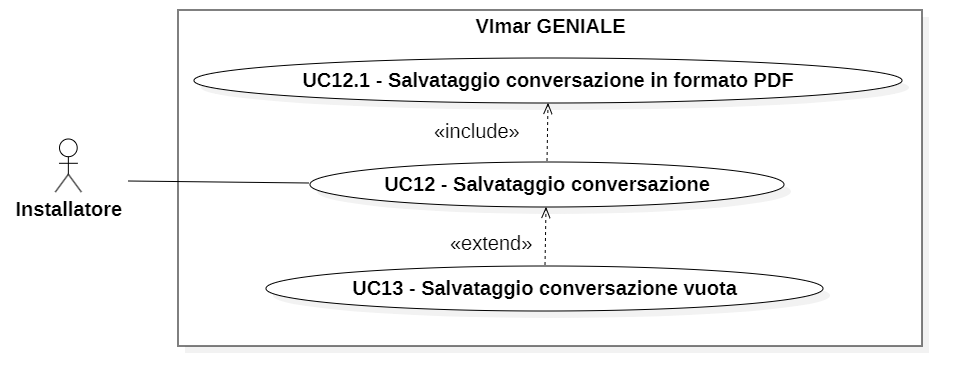
\includegraphics[width=0.8\textwidth]{contents/casi_duso/png/UC12.png}
\caption{UC12, UC12.1 UC13 - Accesso al \textit{cruscotto informativo}\textsubscript{G} }
% \label{fig:UC1a}
\end{figure}

\subuc{Inserimento \textit{username}\textsubscript{G} e \textit{password}\textsubscript{G}}{inserimento_username}
\begin{itemize}
    \item \textbf{Attori coinvolti}: \textit{Amministratore}\textsubscript{G};
    \item \textbf{Descrizione}: Un \textit{amministratore}\textsubscript{G} desidera accedere al \textit{cruscotto informativo}\textsubscript{G} per visualizzare una panoramica di informazioni relative all’utilizzo del \textit{sistema}\textsubscript{G}, dunque inserisce lo \textit{username}\textsubscript{G} e la \textit{password}\textsubscript{G};
    \item \textbf{Precondizioni}: 
        \begin{itemize}
            \item L’\textit{amministratore}\textsubscript{G} ha accesso all’\textit{interfaccia web}\textsubscript{G} del \textit{sistema}\textsubscript{G};
            \item L’\textit{amministratore}\textsubscript{G} è dotato dello \textit{username}\textsubscript{G} e della \textit{password}\textsubscript{G} necessarie ad accedere alla \textit{dashboard}\textsubscript{G}.
        \end{itemize}
    \item \textbf{Postcondizioni}: L’\textit{amministratore}\textsubscript{G} ha inserito lo \textit{username}\textsubscript{G} e la \textit{password}\textsubscript{G}, ovvero le credenziali richieste per l’accesso al \textit{cruscotto informativo}\textsubscript{G};
    \item \textbf{Scenario principale}:
    \begin{enumerate}
    \item L’\textit{amministratore}\textsubscript{G} accede all’\textit{interfaccia web}\textsubscript{G} di Vimar GENIALE;
    \item Inserisce lo \textit{username}\textsubscript{G}.
    \item Inserisce la \textit{password}\textsubscript{G}.
    \end{enumerate}
\end{itemize}


\uc{Inserimento \textit{username}\textsubscript{G} o \textit{password}\textsubscript{G} errati}{inserimento_cred_errati}
\begin{itemize}
    \item \textbf{Attori coinvolti}: \textit{Amministratore}\textsubscript{G};
    \item \textbf{Descrizione}: Un \textit{amministratore}\textsubscript{G} desidera accedere al \textit{cruscotto informativo}\textsubscript{G} per visualizzare una panoramica di informazioni relative all’utilizzo del \textit{sistema}\textsubscript{G}, ma non riesce ad accedere a causa di un errore nell’inserimento dello \textit{username}\textsubscript{G} o della \textit{password}\textsubscript{G};
    \item \textbf{Precondizioni}: 
        \begin{itemize}
            \item L’\textit{amministratore}\textsubscript{G} ha accesso all’\textit{interfaccia web}\textsubscript{G} del \textit{sistema}\textsubscript{G};
            \item L’\textit{amministratore}\textsubscript{G} è dotato delle credenziali necessarie ad accedere alla \textit{dashboard}\textsubscript{G};
            \item Lo \textit{username}\textsubscript{G} o la \textit{password}\textsubscript{G} non sono corretti.
        \end{itemize}
    \item \textbf{Postcondizioni}: Il \textit{sistema}\textsubscript{G} restituisce una risposta che indica il motivo per cui si è verificato l’errore;
    \item \textbf{Scenario principale}:
    \begin{enumerate}
    \item L’\textit{amministratore}\textsubscript{G} accede all’\textit{interfaccia web}\textsubscript{G} di Vimar GENIALE;
    \item Inserisce le proprie credenziali;
    \item Il \textit{sistema}\textsubscript{G} elabora la richiesta e fornisce una risposta che spiega l’inserimento errato delle credenziali;
    \item L’\textit{amministratore}\textsubscript{G} visualizza le informazioni sull’errore che si è verificato.
    \end{enumerate}
\end{itemize}

\uc{Visualizzazione informazioni sulla \textit{dashboard}\textsubscript{G}}{visualizzazione_info_dashboard}
\begin{itemize}
    \item \textbf{Attori coinvolti}: \textit{Amministratore}\textsubscript{G};
    \item \textbf{Descrizione}: Un \textit{amministratore}\textsubscript{G} desidera visualizzare una panoramica di informazioni relative all’utilizzo del \textit{sistema}\textsubscript{G} dal \textit{cruscotto informativo}\textsubscript{G};
    \item \textbf{Precondizioni}: 
        \begin{itemize}
            \item L’\textit{amministratore}\textsubscript{G} ha accesso all’\textit{interfaccia web}\textsubscript{G} del \textit{sistema}\textsubscript{G};
            \item L’\textit{amministratore}\textsubscript{G} è dotato dell’accesso alla \textit{dashboard}\textsubscript{G};
        \end{itemize}
    \item \textbf{Postcondizioni}: Il \textit{sistema}\textsubscript{G} raccoglie le informazioni richieste e le mostra nella \textit{dashboard}\textsubscript{G};
    \item \textbf{Scenario principale}:
    \begin{enumerate}
    \item L’\textit{amministratore}\textsubscript{G} accede all’\textit{interfaccia web}\textsubscript{G} di Vimar GENIALE;
    \item Inserisce le proprie credenziali;
    \item Il \textit{sistema}\textsubscript{G} riceve la richiesta di accesso e \textit{verifica}\textsubscript{G} le credenziali;
    \item L’\textit{amministratore}\textsubscript{G} ottiene l’accesso alla \textit{dashboard}\textsubscript{G};
    \item Il \textit{sistema}\textsubscript{G} mostra le informazioni richieste sul \textit{cruscotto informativo}\textsubscript{G}.
    \end{enumerate}
    \item \textbf{Inclusioni}: 
    \begin{itemize}
        \item UC12 - Accesso al \textit{cruscotto informativo}\textsubscript{G};
        \item UC14.1 - Visualizzazione numero richieste con \textit{conversazione libera}\textsubscript{G};
        \item UC14.2 - Visualizzazione numero richieste con \textit{conversazione guidata}\textsubscript{G};
        \item UC14.3 - Visualizzazione classifica di parole più utilizzate;
        \item UC14.4 - Visualizzazione numero risposte positive dal \textit{sistema}\textsubscript{G} di \textit{feedback}\textsubscript{G};
        \item UC14.5 - Visualizzazione numero negative positive dal \textit{sistema}\textsubscript{G} di \textit{feedback}\textsubscript{G}.
    \end{itemize}
\end{itemize}
\begin{figure}[H]
\centering
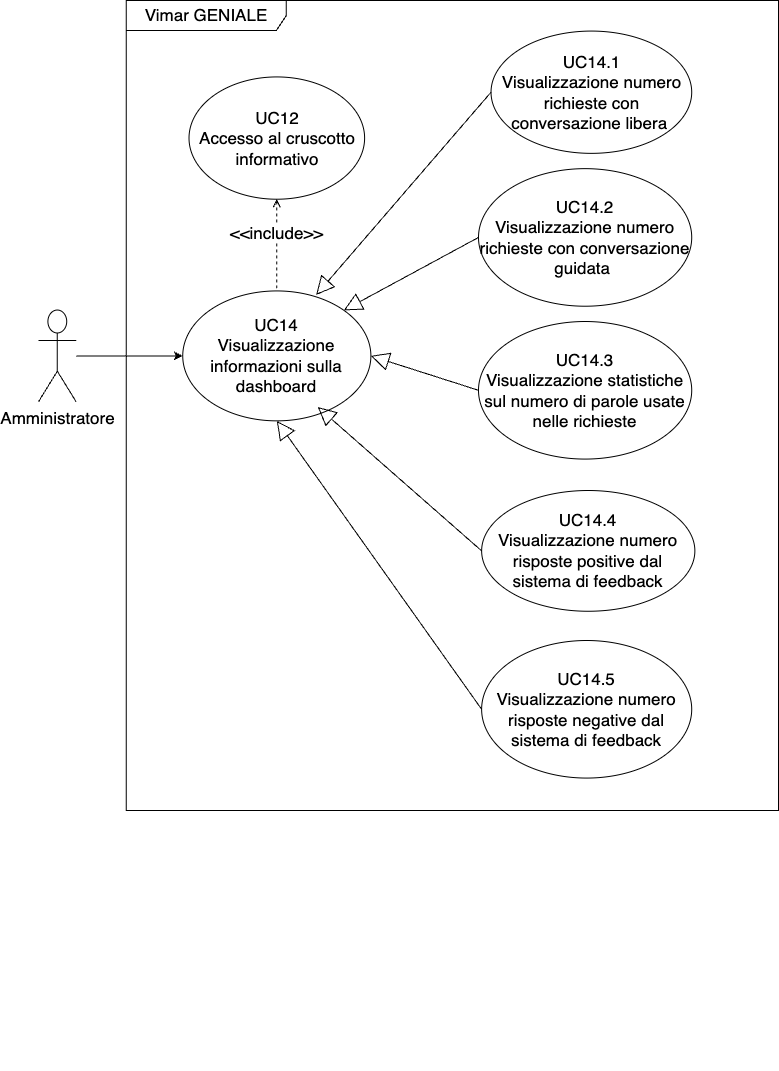
\includegraphics[width=0.8\textwidth]{contents/casi_duso/png/UC14.png}
\caption{UC14, UC14.1, UC14.2, UC14.3, UC14.4, UC14.5 - Visualizzazione informazioni \textit{dashboard}\textsubscript{G}}
% \label{fig:UC1a}
\end{figure}

\subuc{Visualizzazione numero richieste con \textit{conversazione libera}\textsubscript{G}}{visualizzazione_richieste_libere}
\begin{itemize}
    \item \textbf{Attori coinvolti}: \textit{Amministratore}\textsubscript{G};
    \item \textbf{Descrizione}: Un \textit{amministratore}\textsubscript{G} desidera visualizzare dal \textit{cruscotto informativo}\textsubscript{G} il numero delle richieste effettuate con una \textit{conversazione libera}\textsubscript{G};
    \item \textbf{Precondizioni}: 
        \begin{itemize}
            \item L’\textit{amministratore}\textsubscript{G} ha accesso all’\textit{interfaccia web}\textsubscript{G} del \textit{sistema}\textsubscript{G};
            \item L’\textit{amministratore}\textsubscript{G} è dotato dell’accesso alla \textit{dashboard}\textsubscript{G};
        \end{itemize}
    \item \textbf{Postcondizioni}: Il \textit{sistema}\textsubscript{G} raccoglie le informazioni relative al numero delle richieste effettuate con una \textit{conversazione libera}\textsubscript{G} e le mostra nella \textit{dashboard}\textsubscript{G};
    \item \textbf{Scenario principale}:
    \begin{enumerate}
    \item L’\textit{amministratore}\textsubscript{G} accede all’\textit{interfaccia web}\textsubscript{G} di Vimar GENIALE;
    \item Inserisce le proprie credenziali;
    \item Il \textit{sistema}\textsubscript{G} riceve la richiesta di accesso e \textit{verifica}\textsubscript{G} le credenziali;
    \item L’\textit{amministratore}\textsubscript{G} ottiene l’accesso alla \textit{dashboard}\textsubscript{G};
    \item Il \textit{sistema}\textsubscript{G} mostra le informazioni richieste sul \textit{cruscotto informativo}\textsubscript{G}.
    \end{enumerate}
\end{itemize}

\subuc{Visualizzazione numero richieste con \textit{conversazione guidata}\textsubscript{G}}{visualizzazione_richieste_guidate}
\begin{itemize}
    \item \textbf{Attori coinvolti}: \textit{Amministratore}\textsubscript{G};
    \item \textbf{Descrizione}: Un \textit{amministratore}\textsubscript{G} desidera visualizzare dal \textit{cruscotto informativo}\textsubscript{G} il numero delle richieste effettuate con una \textit{conversazione guidata}\textsubscript{G};
    \item \textbf{Precondizioni}: 
        \begin{itemize}
            \item L’\textit{amministratore}\textsubscript{G} ha accesso all’\textit{interfaccia web}\textsubscript{G} del \textit{sistema}\textsubscript{G};
            \item L’\textit{amministratore}\textsubscript{G} è dotato dell’accesso alla \textit{dashboard}\textsubscript{G};
        \end{itemize}
    \item \textbf{Postcondizioni}: Il \textit{sistema}\textsubscript{G} raccoglie le informazioni relative al numero delle richieste effettuate con una \textit{conversazione guidata}\textsubscript{G} e le mostra nella \textit{dashboard}\textsubscript{G};
    \item \textbf{Scenario principale}:
    \begin{enumerate}
    \item L’\textit{amministratore}\textsubscript{G} accede all’\textit{interfaccia web}\textsubscript{G} di Vimar GENIALE;
    \item Inserisce le proprie credenziali;
    \item Il \textit{sistema}\textsubscript{G} riceve la richiesta di accesso e \textit{verifica}\textsubscript{G} le credenziali;
    \item L’\textit{amministratore}\textsubscript{G} ottiene l’accesso alla \textit{dashboard}\textsubscript{G};
    \item Il \textit{sistema}\textsubscript{G} mostra le informazioni richieste sul \textit{cruscotto informativo}\textsubscript{G}.
    \end{enumerate}
\end{itemize}

\subuc{Visualizzazione classifica di parole più utilizzate}{visualizzazione_statistiche_parole}
\begin{itemize}
    \item \textbf{Attori coinvolti}: \textit{Amministratore}\textsubscript{G};
    \item \textbf{Descrizione}: Un \textit{amministratore}\textsubscript{G} desidera visualizzare dal \textit{cruscotto informativo}\textsubscript{G} la classifica delle parole più utilizzate con relativa percentuale rispetto al numero totale delle parole utilizzate nelle richieste;
    \item \textbf{Precondizioni}: 
        \begin{itemize}
            \item L’\textit{amministratore}\textsubscript{G} ha accesso all’\textit{interfaccia web}\textsubscript{G} del \textit{sistema}\textsubscript{G};
            \item L’\textit{amministratore}\textsubscript{G} è dotato dell’accesso alla \textit{dashboard}\textsubscript{G};
        \end{itemize}
    \item \textbf{Postcondizioni}: Il \textit{sistema}\textsubscript{G} raccoglie le informazioni relative alla classifica delle parole più utilizzate nelle richieste e la mostra nella \textit{dashboard}\textsubscript{G};
    \item \textbf{Scenario principale}:
    \begin{enumerate}
    \item L’\textit{amministratore}\textsubscript{G} accede all’\textit{interfaccia web}\textsubscript{G} di Vimar GENIALE;
    \item Inserisce le proprie credenziali;
    \item Il \textit{sistema}\textsubscript{G} riceve la richiesta di accesso e \textit{verifica}\textsubscript{G} le credenziali;
    \item L’\textit{amministratore}\textsubscript{G} ottiene l’accesso alla \textit{dashboard}\textsubscript{G};
    \item Il \textit{sistema}\textsubscript{G} mostra le informazioni richieste sul \textit{cruscotto informativo}\textsubscript{G}.
    \end{enumerate}
\end{itemize}

\subuc{Visualizzazione numero risposte positive dal \textit{sistema}\textsubscript{G} di \textit{feedback}\textsubscript{G}}{visualizzazione_risposte_positive}
\begin{itemize}
    \item \textbf{Attori coinvolti}: \textit{Amministratore}\textsubscript{G};
    \item \textbf{Descrizione}: Un \textit{amministratore}\textsubscript{G} desidera visualizzare dal \textit{cruscotto informativo}\textsubscript{G} il numero delle risposte positive dal \textit{sistema}\textsubscript{G} di \textit{feedback}\textsubscript{G};
    \item \textbf{Precondizioni}: 
        \begin{itemize}
            \item L’\textit{amministratore}\textsubscript{G} ha accesso all’\textit{interfaccia web}\textsubscript{G} del \textit{sistema}\textsubscript{G};
            \item L’\textit{amministratore}\textsubscript{G} è dotato dell’accesso alla \textit{dashboard}\textsubscript{G};
        \end{itemize}
    \item \textbf{Postcondizioni}: Il \textit{sistema}\textsubscript{G} raccoglie le informazioni relative al numero delle risposte positive dal \textit{sistema}\textsubscript{G} di \textit{feedback}\textsubscript{G} e le mostra nella \textit{dashboard}\textsubscript{G};
    \item \textbf{Scenario principale}:
    \begin{enumerate}
    \item L’\textit{amministratore}\textsubscript{G} accede all’\textit{interfaccia web}\textsubscript{G} di Vimar GENIALE;
    \item Inserisce le proprie credenziali;
    \item Il \textit{sistema}\textsubscript{G} riceve la richiesta di accesso e \textit{verifica}\textsubscript{G} le credenziali;
    \item L’\textit{amministratore}\textsubscript{G} ottiene l’accesso alla \textit{dashboard}\textsubscript{G};
    \item Il \textit{sistema}\textsubscript{G} mostra le informazioni richieste sul \textit{cruscotto informativo}\textsubscript{G}.
    \end{enumerate}
\end{itemize}

\subuc{Visualizzazione numero risposte negative dal \textit{sistema}\textsubscript{G} di \textit{feedback}\textsubscript{G}}{visualizzazione_risposte_negative}
\begin{itemize}
    \item \textbf{Attori coinvolti}: \textit{Amministratore}\textsubscript{G};
    \item \textbf{Descrizione}: Un \textit{amministratore}\textsubscript{G} desidera visualizzare dal \textit{cruscotto informativo}\textsubscript{G} il numero delle risposte negative dal \textit{sistema}\textsubscript{G} di \textit{feedback}\textsubscript{G};
    \item \textbf{Precondizioni}: 
        \begin{itemize}
            \item L’\textit{amministratore}\textsubscript{G} ha accesso all’\textit{interfaccia web}\textsubscript{G} del \textit{sistema}\textsubscript{G};
            \item L’\textit{amministratore}\textsubscript{G} è dotato dell’accesso alla \textit{dashboard}\textsubscript{G};
        \end{itemize}
    \item \textbf{Postcondizioni}: Il \textit{sistema}\textsubscript{G} raccoglie le informazioni relative al numero delle risposte negative dal \textit{sistema}\textsubscript{G} di \textit{feedback}\textsubscript{G} e le mostra nella \textit{dashboard}\textsubscript{G};
    \item \textbf{Scenario principale}:
    \begin{enumerate}
    \item L’\textit{amministratore}\textsubscript{G} accede all’\textit{interfaccia web}\textsubscript{G} di Vimar GENIALE;
    \item Inserisce le proprie credenziali;
    \item Il \textit{sistema}\textsubscript{G} riceve la richiesta di accesso e \textit{verifica}\textsubscript{G} le credenziali;
    \item L’\textit{amministratore}\textsubscript{G} ottiene l’accesso alla \textit{dashboard}\textsubscript{G};
    \item Il \textit{sistema}\textsubscript{G} mostra le informazioni richieste sul \textit{cruscotto informativo}\textsubscript{G}.
    \end{enumerate}
\end{itemize}



\uc{Richiesta di argomento proibito}{argomento_proibito}
\begin{itemize}
    \item \textbf{Attori coinvolti}: Installatore;
    \item \textbf{Descrizione}: L’installatore richiede argomenti proibiti al \textit{sistema}\textsubscript{G} (e.g. politica, finanza, pornografia, ...);
    \item \textbf{Precondizioni}: 
        \begin{itemize}
            \item L’installatore ha accesso all’\textit{interfaccia web}\textsubscript{G} del \textit{sistema}\textsubscript{G};
            \item L’installatore ha accesso ad una conversazione memorizzabile nel \textit{sistema}\textsubscript{G};
            \item La domanda posta non riguarda argomenti proibiti.
        \end{itemize}
    \item \textbf{Postcondizioni}: Il \textit{sistema}\textsubscript{G} restituisce una risposta che indica il motivo per cui si è verificato l’errore;
    \item \textbf{Scenario principale}:
    \begin{enumerate}
    \item L’installatore accede all’\textit{interfaccia web}\textsubscript{G} di Vimar GENIALE;
    \item Inserisce una domanda inconsistente, che non ha a che vedere con prodotti \textit{VIMAR}\textsubscript{G};
    \item Il \textit{sistema}\textsubscript{G} elabora la richiesta e fornisce una risposta che spiega la causa dell'errore riscontrato;
    \item L’installatore visualizza le informazioni sull’errore che si è verificato;
    \end{enumerate}
     \item \textbf{Inclusioni}: UC6 - Ricerca informazioni sui prodotti con conversazione libera.
\end{itemize}

\uc{Domanda al sistema\textsubscript{G}}{domanda}
\begin{itemize}
    \item \textbf{Attori coinvolti}: Installatore;
    \item \textbf{Descrizione}: L’installatore inserisce una domanda;
    \item \textbf{Precondizioni}: 
        \begin{itemize}
            \item L’installatore ha accesso all’\textit{interfaccia web}\textsubscript{G} del \textit{sistema}\textsubscript{G};
            \item L’installatore ha accesso ad una conversazione memorizzabile nel \textit{sistema}\textsubscript{G};
            \item L'installatore ha inviato una domanda al \textit{sistema}\textsubscript{G};
            \item La domanda posta non riguarda argomenti proibiti.
        \end{itemize}
    \item \textbf{Postcondizioni}: Il \textit{sistema}\textsubscript{G} restituisce una risposta;
    \item \textbf{Scenario principale}:
    \begin{enumerate}
    \item L’installatore accede all’\textit{interfaccia web}\textsubscript{G} di Vimar GENIALE;
    \item Inserisce una domanda che ha a che vedere con prodotti \textit{VIMAR}\textsubscript{G} e non con argomenti proibiti o sconosciuti;
    \item Il \textit{sistema}\textsubscript{G} elabora la richiesta e fornisce una risposta;
    \item L’installatore visualizza le informazioni restituite;
    \end{enumerate}
\end{itemize}
\begin{figure}[H]
\centering
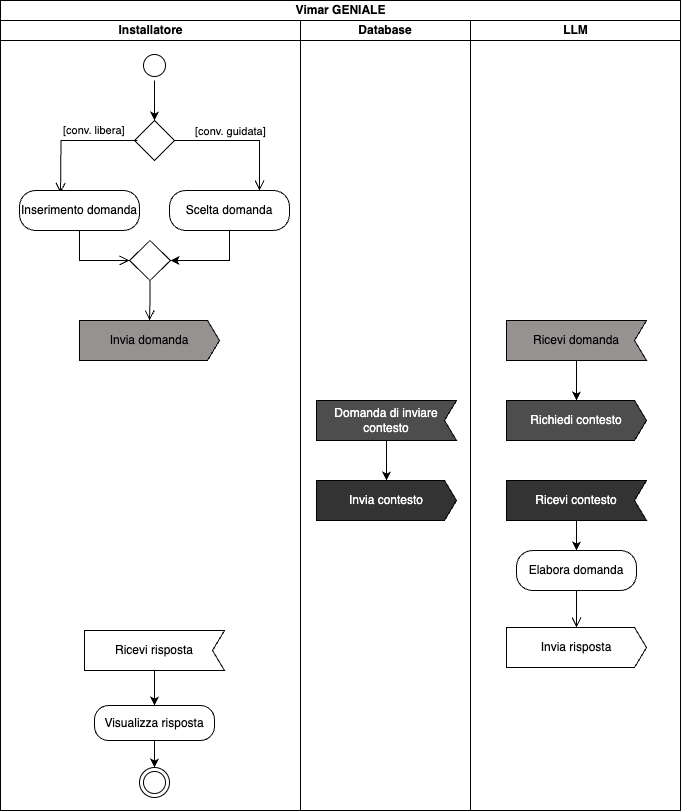
\includegraphics[width=0.8\textwidth]{contents/casi_duso/png/UC16_activity.png}
\caption{UC16 - Domanda al \textit{sistema}\textsubscript{G}}
% \label{fig:UC1a}
\end{figure}

\uc{Richiesta di uno schema o immagine}{domanda_immagine}
\begin{itemize}
    \item \textbf{Attori coinvolti}: Installatore;
    \item \textbf{Descrizione}: L’installatore inserisce una domanda la cui risposta prevede uno schema elettrico o un'immagine;
    \item \textbf{Precondizioni}: 
        \begin{itemize}
            \item L’installatore ha accesso all’\textit{interfaccia web}\textsubscript{G} del \textit{sistema}\textsubscript{G};
            \item L’installatore ha accesso ad una conversazione memorizzabile nel \textit{sistema}\textsubscript{G};
            \item L'installatore ha inviato una domanda al \textit{sistema}\textsubscript{G};
            \item La risposta alla domanda posta necessita, per essere completa, si uno schema elettrico o di un'immagine.
        \end{itemize}
    \item \textbf{Postcondizioni}: Il \textit{sistema}\textsubscript{G} restituisce una risposta con l'immagine o lo schema corretto;
    \item \textbf{Scenario principale}:
    \begin{enumerate}
    \item L’installatore accede all’\textit{interfaccia web}\textsubscript{G} di Vimar GENIALE;
    \item Inserisce una domanda che ha a che vedere con prodotti \textit{VIMAR}\textsubscript{G};
    \item Il \textit{sistema}\textsubscript{G} elabora la richiesta e fornisce una risposta inserendo uno schema o di un'immagine di cui la risposta ha bisogno per essere esaustiva;
    \item L’installatore visualizza le informazioni restituite;
    \end{enumerate}
    \item \textbf{Generalizzazioni}: UC6 - Ricerca informazioni sui prodotti con \textit{conversazione libera}\textsubscript{G}.  
\end{itemize}



\uc{ Digitazione della Domanda}{digita_domanda}
\begin{itemize}
    \item \textbf{Attori coinvolti}: Installatore;
    \item \textbf{Descrizione}: L’installatore inserisce una domanda;
    \item \textbf{Precondizioni}: 
        \begin{itemize}
            \item L’installatore ha accesso all’\textit{interfaccia web}\textsubscript{G} del \textit{sistema}\textsubscript{G};
        \end{itemize}
    \item \textbf{Postcondizioni}: L'installatore invia la domanda al \textit{sistema}\textsubscript{G};
    \item \textbf{Scenario principale}:
    \begin{enumerate}
    \item L’installatore accede all’\textit{interfaccia web}\textsubscript{G} di Vimar GENIALE;
    \item Inserisce una domanda;
    \item Il \textit{sistema}\textsubscript{G} riceve la domanda ed inizia ad elaborarla;
    \end{enumerate}
    \item \textbf{Estensioni}: UC7 - Superamento limite caratteri del messaggio.
\end{itemize}


\newpage
\section{Requisiti}
In questa sezione verranno elencati tutti i requisiti specificati nel \textit{capitolato}\textsubscript{G}, organizzandoli in categorie distinte per una maggiore chiarezza. Ogni \textit{requisito}\textsubscript{G} è identificato in modo univoco da un codice, strutturato secondo un formato predefinito, che ne facilita la consultazione e il riferimento all'interno della \textit{documentazione}\textsubscript{G} con il seguente formato: 
\begin{center}
\textbf{R[Tipo].[Importanza].[Codice]}
\end{center}
dove:
\begin{itemize}
    \item \textbf{Codice:} un numero progressivo a tre cifre che parte dal numero 001.
    \item \textbf{Tipo:} la tipologia di \textit{requisito}\textsubscript{G} che può essere tra le seguenti:
    \begin{itemize}[label=-]
        \item \textbf{F (funzionale):} Una funzione di \textit{sistema}\textsubscript{G} descrive il modo in cui un \textit{sistema}\textsubscript{G} utilizza determinati ingressi per generare specifiche uscite, seguendo una logica o una regola prestabilita che definisce il suo comportamento.
        \item \textbf{Q (qualità):} definisce le caratteristiche di qualità del prodotto \textit{software}\textsubscript{G}.
        \item \textbf{V (vincolo):} specifica i limiti e le restrizioni imposte dal \textit{capitolato}\textsubscript{G}, che il prodotto \textit{software}\textsubscript{G} deve rispettare.
\end{itemize}
    \item \textbf{Importanza:} la priorità viene assegnata al \textit{requisito}\textsubscript{G} con:
    \begin{itemize}
     \item \textbf{O}: \textit{requisito}\textsubscript{G} obbligatorio che deve essere soddisfatto per la realizzazione del prodotto \textit{software}\textsubscript{G};
        \item \textbf{D}: \textit{requisito}\textsubscript{G} desiderabile il cui soddisfacimento è apprezzato dal \textit{committente}\textsubscript{G};
        \item \textbf{P}: \textit{requisito}\textsubscript{G} facoltativo, la cui realizzazione è totalmente a discrezione del team in base all'andamento del progetto.
    \end{itemize}
\end{itemize}
In alcuni casi sarà specificato nella colonna delle fonti se il \textit{requisito}\textsubscript{G} è stato esplicitamente indicato nel \textit{Capitolato}\textsubscript{G} oppure se è stato dedotto implicitamente da altri requisiti obbligatori. In quest’ultimo caso, si farà riferimento a un \textit{requisito}\textsubscript{G} interno.
\subsection{Registro di Funzionalità}
\begin{table}[H]
    \begin{tabular}{|C{2.7cm}|L{7.2cm}|C{2.7cm}|C{2cm}|}
        \hline
        \textbf{ID requisito} & \textbf{Descrizione} & \textbf{Importanza} & \textbf{Fonti}  \\
        \hline
        RF.O.1 & Il sistema deve permettere all'installatore di effettuare ricerche testuali e ricevere informazioni dettagliate sui prodotti Vimar. & Obbligatorio & Capitolato \\
        \hline
        RF.O.2 & Il sistema deve prevedere un sistema di autenticazione tramite password per l'accesso alla dashboard per amministratori. & Obbligatorio & UC12 \\
        \hline
        RF.O.3 & Il cruscotto informativo deve includere una sezione per la visualizzazione di statistiche di utilizzo. & Obbligatorio & UC14 \\
        \hline
        RF.O.4 & Il sistema deve permettere agli utenti di fornire un feedback positivo o negativo dopo ogni risposta ricevuta. & Obbligatorio & UC14 \\
        \hline
        RF.O.5 & Il sistema deve essere in grado di identificare e bloccare le richieste che riguardano argomenti non pertinenti ai prodotti VIMAR. & Obbligatorio & UC15 \\
        \hline
        RF.D.6 & Il sistema potrebbe includere la possibilità di visualizzare link di riferimento alle fonti delle informazioni fornite. & Desiderabile & Capitolato \\
        \hline
        RF.P.7 & Il sistema deve fornire un'interfaccia con menu e sottomenù per costruire richieste specifiche in conversazioni guidate & Opzionale & Capitolato\\
        \hline
        RF.O.8 & Il sistema deve consentire solo conversazioni pertinendi ai prodotti Vimar e bloccare conversazioni su argomenti proibiti & Obbligatorio & Capitolato \\
        \hline
        \end{tabular}

\end{table}
\subsection{Requisiti di Qualità}
\begin{longtable}{|C{2.7cm}|L{7.2cm}|C{2.7cm}|C{2cm}|}
        \hline
        \textbf{ID requisito} & \textbf{Descrizione} & \textbf{Importanza} & \textbf{Fonti}  \\
        \hline
       
        \hline
        RQ.D.001 & L'interfaccia utente del sistema potrebbe essere responsive, adattandosi a diversi dispositivi. & Desiderabile & Capitolato \\
        \hline
        RQ.O.002 & Il sistema deve essere progettato per essere facilmente eseguibile su altri dispositivi utilizzando la tecnologia dei container. & Obbligatorio & Capitolato \\
        
        \hline
        RQ.O.003 & \'E necessario fornire un documento che descriva le attività di bug\textsubscript{G} reporting effettuate. & Obbligatorio & Interno \\
        \hline
        RQ.O.004 & Il progetto deve essere svolto seguendo le regole contenute nel documento Norme di Progetto. & Obbligatorio & Interno \\
        \hline
        RQ.O.005 & \'E necessario fornire al proponente il codice sorgente dell'applicativo in un
        repository\textsubscript{G} GitHub. & Obbligatorio & Interno \\
        \hline
        RQ.O.006 & \'E necessario fornire il Manuale Utente dell'applicativo. & Obbligatorio & Interno \\
        \hline
        
        


\end{longtable}
\subsection{Requisiti di Vincolo}

\begin{longtable}{|C{2.7cm}|L{7.2cm}|C{2.7cm}|C{2cm}|}
        \hline
    \textbf{ID requisito} & \textbf{Descrizione} & \textbf{Importanza} & \textbf{Fonti}  \\
    \hline
           RV.O.001 & Il sistema deve integrare un modello AI (LLM) open source. & Obbligatorio & Capitolato \\
          \hline 
          RV.O.002 & L’infrastruttura Cloud deve utilizzare Docker insieme a Docker Compose, al fine di rispettare il principio di Infrastructure as Code. & Obbligatorio & Capitolato \\
           \hline
          RV.D.003 & L'applicativo può essere ospitato su AWS. & Desiderabile & Capitolato \\
          \hline
          RV.O.004 & Il modello AI (LLM) deve essere Open Source.
         & Obbligatorio & Capitolato \\
        \hline
        RV.O.005 & Il componente di interrogazione deve essere in grado di interfacciarsi con il sistema di indicizzazione e con il modello AI (LLM).
         & Obbligatorio & Capitolato \\
        \hline
        RV.O.006 & Il componente di interrogazione deve poter essere contattato da un altro servizio sotto-forma di API autenticata (ad esempio tramite API-KEY)
         & Obbligatorio & Capitolato \\
        \hline
        RV.O.007 &  L’infrastruttura deve utilizzare la tecnologia dei container.
         & Obbligatorio & Capitolato \\
        \hline
         RV.O.008 & Il risultato atteso è che la parte applicativa possa essere costruita e replicata con un solo comando.
         & Obbligatorio & Capitolato \\
        \hline
        RV.O.009 & Il repository di lavoro deve essere versionato tramite Git e deve essere pubblicamente accessibile.
         & Obbligatorio & Capitolato \\
        \hline
        RV.O.010 & La licenza per i sorgenti dovrà essere open source.
         & Obbligatorio & Capitolato \\
        \hline
        RV.O.011 & Il modello AI (LLM) dovrà fare uso dell’approccio RAG.
         & Obbligatorio & Capitolato \\
        \hline
        RV.O.012 & L’applicazione deve essere compatibile con il browser Chrome dalla
        versione 108.
         & Obbligatorio & Interno \\
        \hline
        RV.O.013 & L’applicazione deve essere compatibile con il browser Edge dalla versione 94.0.992.31.
         & Obbligatorio & Interno \\
        \hline
        RV.O.014 & L’applicazione deve essere compatibile con il browser Opera dalla
        versione 95.
         & Obbligatorio & Interno \\
        \hline
        RV.O.015 & L’applicazione deve essere compatibile con il browser Firefox dalla
versione 109.
         & Obbligatorio & Interno \\
        \hline
        RV.O.016 & L’applicazione deve essere compatibile con il browser Safari dalla
versione 16.
         & Obbligatorio & Interno \\
        \hline


        
        

\end{longtable}
\newpage
\section{Tracciamento Requisiti}
\begin{table}[H]
\centering
    \begin{tabular}{|C{3.0cm}|C{3.0cm}|}
        \hline
         \textbf{Fonte} &
         \textbf{ID requisito}   
          \\
          \hline
          Capitolato & R-XXX-X-X \\
          \hline 
          Interno & R-XXX-X-X \\
          \hline
    \end{tabular}
\end{table}
\subsection{Riepilogo}
\begin{table}[H]
\centering
    \begin{tabular}{|C{3.0cm}|C{2.5cm}|C{2.5cm}|C{2.5cm}|}
        \hline
         \textbf{Tipologia} &
         \textbf{Obbligatori} & 
         \textbf{Desiderabili} &
         \textbf{Funzionali} 
          \\
          \hline
          \textbf{Funzionali} & 00 & 00 & 00 \\
          \hline 
          \textbf{Qualità} & 00 & 00 & 00\\
          \hline
          \textbf{Vincolo} & 00 & 00 & 00\\
          \hline
    \end{tabular}
\end{table}
\subsection{Conclusioni}
\newpage
\end{document}
